\chapter{Linear Algebra Based Approach to Context-Free Path Querying}\label{ch:ch2}
%В этой главе представлен подход к решению класса задач по поиску путей в графе с ограничениями, заданными КС-языком, с помощью методов линейной алгебры. Т.е. на вход предлагаемый подход получает описание задачи указанного класса, а на выходе выдает алгоритм и некоторые другие артефакты. Несмотря на то, что полностью детерминированную процедуру для создания таких алгоритмов создать не удаётся, видится целесообразным аккумулировать успешный опыт создания ряда алгоритмов этого класса в виде предлагаемого ниже подхода. Этот подход может быть использован как руководство, он также содержит успешные примеры и отсылки к необходимым теоретическим результатам и программным библиотекам. Но он не заменяет акт творческого включения и удачи~--- это создателям алгоритмов для решения задач из указанного класса придётся обеспечить самостоятельно.
This chapter is devoted to the linear algebra based approach to CFPQ. The proposed approach gets a CFPQ problem as input, and returns a CFPQ algorithm and some other artifacts. Despite the fact that it is not possible to create a completely deterministic procedure for creating such algorithms, it seems appropriate to accumulate successful experience in creating a number of CFPQ algorithms in the form of the approach proposed below. This approach can be used as a guide, it also contains successful examples and links to required theoretical results and software libraries.%But it does not replace the act of creative inclusion and luck that the creators of such algorithms will need.

%В начале главы предлагается детальное описание предлагаемого подхода. После этого демонстрируется его использование для частного случая задачи поиска путей в графе с заданными КС-ограничениями, в котором ограничения задаются регулярными языками. В конце проведён анализ применимости и ограничений предложенного подхода.
The chapter begins with a detailed description of the proposed approach. After that, this approach is applied for a partial case of the CFPQ problem, in which the constraints are given by regular languages. At the end, the applicability and limitations of the proposed approach are analyzed.

\section{Description of the Approach}
%Обобщая опыт Лэсли Вэлианта создания матричного алгоритма синтаксического анализа строк, а также подхода \textit{Algebraic Path Problem}, в данном диссертационном исследовании предлагается подход для решения задач поиска путей в графе с КС-ограничениями с помощью методов линейной алгебры.
Summarizing the experience of Leslie Valiant in creating a matrix-based algorithm for parsing strings, as well as the \textit{algebraic path problems} approach, an approach to solve CFPQ problem using linear algebra methods is provided.

%Схема предлагаемого подхода изображена на~\cref{fig:schema}. В качестве фундамента выступают знания из следующих областей: линейная алгебра, теория формальных языков и теория графов. Аппарат линейной алгебры предоставляет: алгоритмы вычисления операций над матрицами и векторами, с помощью которых будет производиться анализ графов; методы решения систем линейных уравнений (такие системы могут возникнуть в матричной форме в процессе построения алгоритма анализа графа); теоретические свойства таких алгоритмов и методов, которые будут во многом определять теоретические свойства результирующего алгоритма; практические результаты в виде готовых высокопроизводительных библиотек линейной алгебры, которые будут использованы в реализации построенного алгоритма. Из теории графов используются: способы представления информации о графах и их связь с объектами линейной алгебры; существующие алгоритмы обхода и поиска путей в графе, которые послужат основой для алгоритмов поиска путей в графе с заданными КС-ограничениями; успешный опыт решения задач анализа графов с помощью методов линейной алгебры, который хорошо описан в книге~\cite{kepner2011graph}, а для задач поиска путей в графе собран в виде подхода \textit{Algebraic Path Problem}~\cite{rote1990path,baras2010path,chen1992parallel,lengauer1991unstructured}; практический опыт применения методов линейной алгебры к задачам анализа графов, который представлен в виде стандарта GraphBLAS~\cite{graphblas} и его реализаций. В свою очередь, теория формальных языков предлагает: способы описания КС-языков (формальные грамматики, конечные автоматы, рекурсивные автоматы), которые будут применены в построенном алгоритме для описания КС-ограничений на пути в графе; алгоритмы преобразования этих представлений (перевод формальных грамматик в нормальные формы, минимизация количества состояний конечных автоматов), упрощающие заданные КС-ограничения, которые позволят использовать более простые и эффективные операции для проверки путей на соответствие этим ограничениям в процессе анализа графа.
A schema of the proposed approach is shown in Figure~\ref{fig:schema}. The background of the approach is knowledge from the following areas: the linear algebra, the formal language theory, and the graph theory. The apparatus of the linear algebra provides: algorithms for calculating operations on matrices and vectors that can be used for the graph analysis; methods for solving systems of linear equations (such systems may arise in the matrix form during the process of constructing a graph analysis algorithm); theoretical properties of such algorithms and methods, which will mainly determine the theoretical properties of the resulting algorithm; practical results in the form of existing high-performance linear algebra libraries that will be used in the constructed algorithm implementation. The graph theory provides the following: various graph representations and their connection with linear algebra objects; existing traversal and path querying algorithms, which will serve as the basis for the CFPQ algorithms; successful experience in solving graph analysis problems using linear algebra methods, which is well described in the book~\cite{kepner2011graph}, and for the path querying problems is collected as an approach \textit{algebraic path problems}~\cite{rote1990path,baras2010path, chen1992parallel,lengauer1991unstructured}; practical experience in applying linear algebra methods to graph analysis problems, which is presented in the form of the GraphBLAS~\cite{graphblas} standard and its implementations. In turn, the formal language theory offers: methods for describing CFLs (formal grammars, recursive automata), which will be used in the constructed algorithm to describe the context-free path constraints; normal forms of CFGs and algorithms for transforming grammars into these normal forms, which will allow one to use simpler derivation rules to describe path constraints.

As input, the proposed approach receives a CFPQ problem. Such problem has many formulations and may differ in the following dimensions:
\begin{itemize}
    \item according to the type of the required information about the paths (reachability problem, single-path query semantics, all-path query semantics);
    \item by the sets of initial and final vertices of the desired paths (searching for paths: between all vertices, with a fixed set of initial vertices, with one initial and one final vertex, etc.);
    \item by the presence of additional constraints on the desired paths (searching for shortest paths, for simple paths, etc.).
\end{itemize}

\begin{figure}
    \centering
	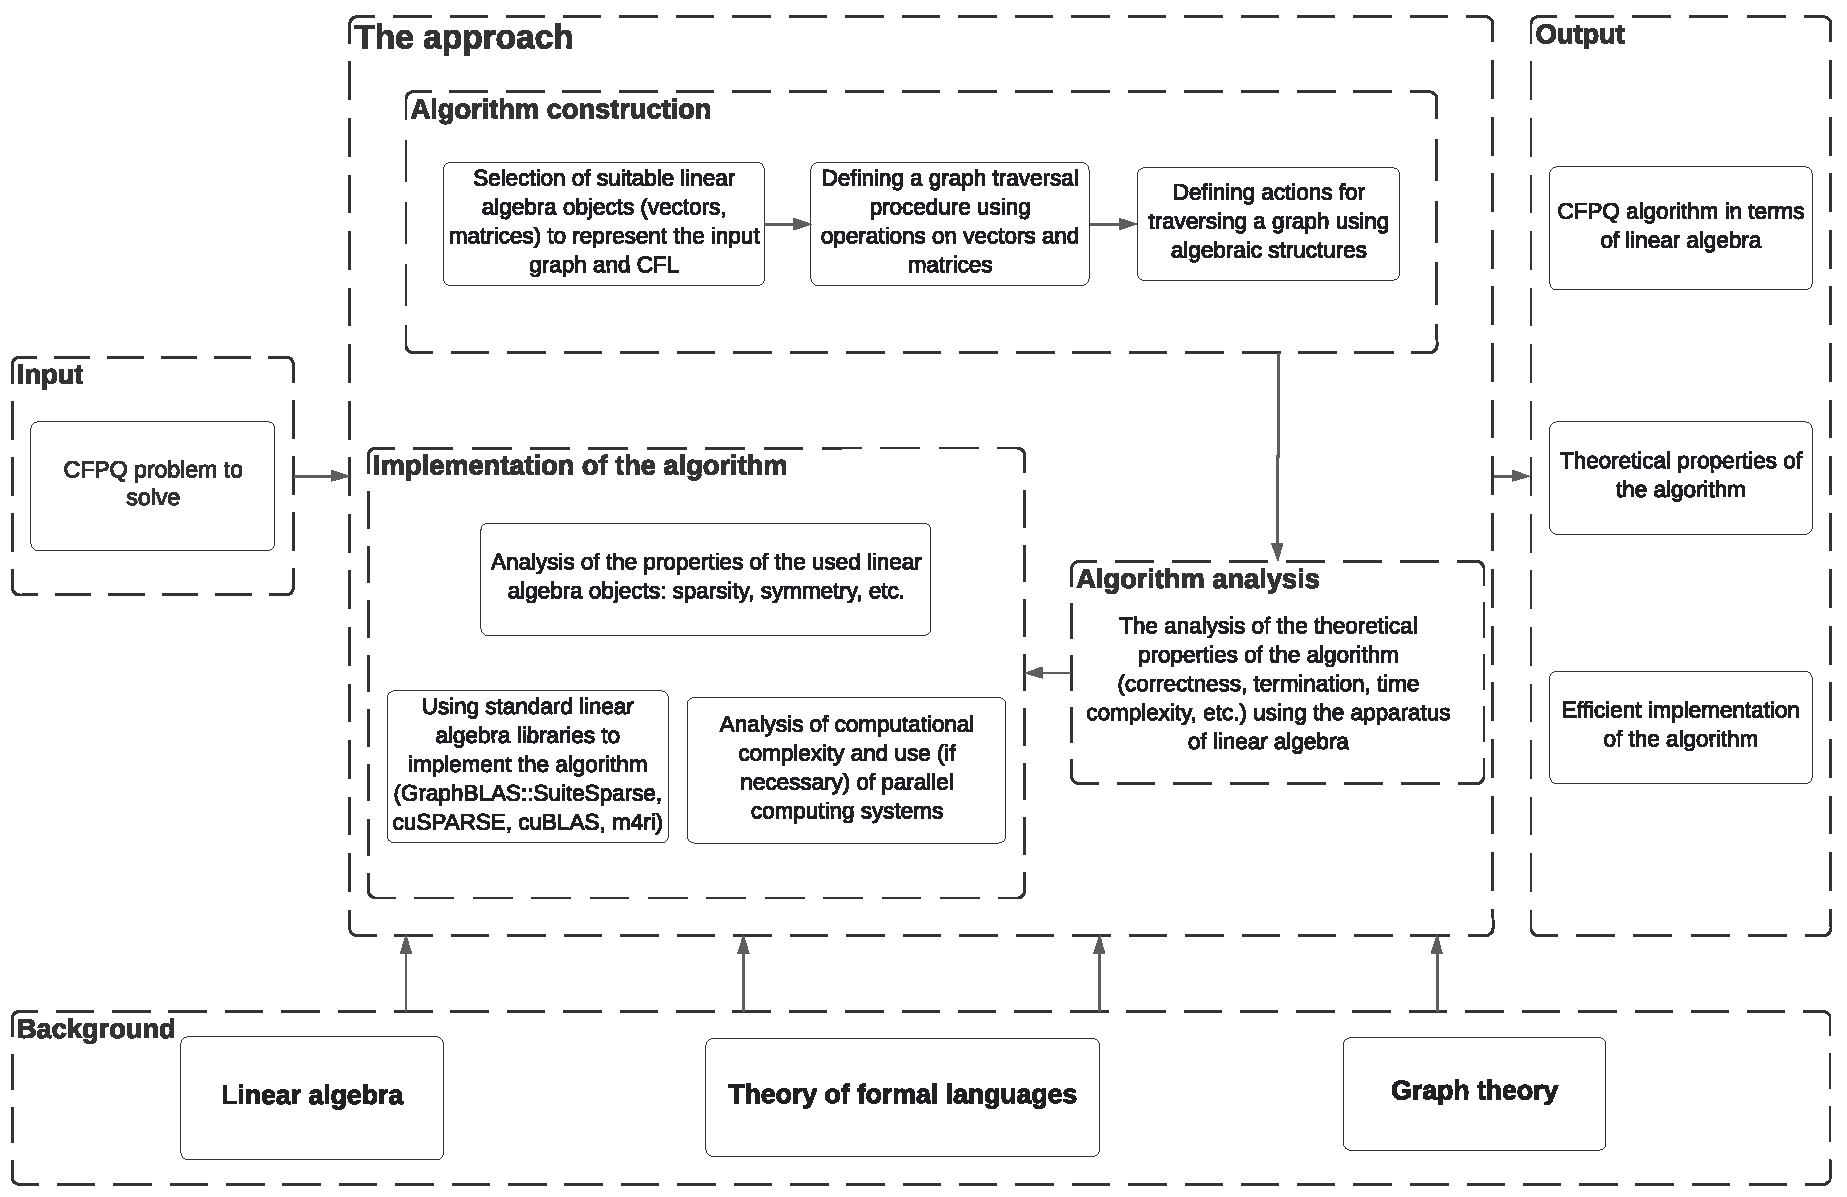
\includegraphics[width = 17.7cm]{Dissertation/images/schema_eng.pdf}
	\caption{A schema of the linear algebra based approach to CFPQ}
	\label{fig:schema}
\end{figure}

%Стоит отметить, что решаемая задача может иметь практическую или теоретическую направленность. Например, при практической направленности целью применения предлагаемого подхода может быть получение высокопроизводительной реализации для решения поставленной задачи анализа графов. А при теоретической направленности основным результатом может являться получение алгоритма, который обладает некоторыми уникальными теоретическими свойствами.
Note that the problem being solved may have a practical or theoretical purpose. For example, with a practical purpose, the goal of applying the proposed approach is to obtain a high-performance implementation of the graph analysis algorithm. And with a theoretical purpose, the main result is to obtain an algorithm that has some unique theoretical properties.

%Также при постановке решаемой задачи может указываться некоторая дополнительная информация про анализируемые графы и используемые КС-ограничения. Например, может быть известна степень разреженности графов или их особый вид (например, что на вход алгоритму будут подаваться только ацикличные графы). Это, в свою очередь, позволит использовать те или иные специфические структуры для хранения информации о графах, а также операции над этими структурами. Для хранения матриц смежности разреженных графов следует выбирать соответствующие разреженные форматы CSR, CSC, COO. А в случае ацикличности графов~--- их матрицы смежности будут иметь треугольный вид, что уменьшит сложность вычисления некоторых операций над ними. Например, первый этап метода Гаусса для решения системы линейных уравнений может быть пропущен, так как он приводит матрицу к треугольной форме. А такая операция, как вычисление транзитивного замыкания для треугольной матрицы имеет сложность, равную сложности вычисления одного умножения матриц. Аналогично, могут быть учтены особенности КС-языков, используемых в качестве КС-ограничений, для поиска наиболее подходящей структуры хранения этих ограничений и операций над этой структурой. Так, если перевод формальной грамматики для заданного КС-языка приводит к слишком значительному увеличению размеров этой грамматики, то целесообразно вместо такой трансформации использовать представление КС-языка в виде рекурсивного автомата. Кроме того, если заданные КС-ограничения соответствуют некоторому подклассу класса КС-языков (например, регулярным языкам), то целесообразно использовать соответствующие более простые структуры (например, конечные автоматы) для описания таких ограничений.
Also, some additional information about the analyzed graphs and the used context-free path constraints can be indicated. For example, the input graph sparsity or special form of the input graph may be known (for example, that only acyclic graphs will be given to the algorithm as input). This, in turn, allows one to use specific structures to store information about graphs, as well as operations on these structures. To store adjacency matrices of sparse graphs, one should choose the appropriate sparse formats CSR, CSC, COO. And in the case of acyclicity of graphs their adjacency matrices will have a triangular form that will reduce the complexity of calculating some operations on them. For example, the first step of the Gauss-Jordan elimination for solving a system of linear equations can be skipped, since it transforms the matrix to a triangular form. And such an operation as the transitive closure calculation for a triangular matrix has a complexity equal to the complexity of calculating a single matrix multiplication. Similarly, the properties of the CFLs used as path constraints can be taken into account in order to find the most appropriate structure for storing these constraints. So, if the normalization of a formal grammar for a given CFL leads to a significant increase of the grammar size then it is advisable to use the representation of the CFL in the form of a recursive automaton. In addition, if the given constraints correspond to some subclass of the class of CFLs (for example, regular languages) then it is advisable to use the corresponding simpler structures (for example, finite automata) to describe such constraints.

The proposed approach is divided into the following parts:
\begin{itemize}
    \item a construction of a CFPQ algorithm in terms of linear algebra;
    \item an analysis of the theoretical properties of the constructed algorithm and the given problem;
    \item an implementation of the constructed algorithm.
\end{itemize}

%Важной частью предлагаемого подхода является само построение алгоритма. Как и при решении других задач анализа графов, ключевым здесь является выбор подходящих объектов линейной алгебры (векторов, матриц) для представления информации о графах. Также подобные объекты можно использовать для представления КС-ограничений путём сведения КС-языков к рекурсивным автоматам~\cite{alur2005analysis} с последующим представлением этих автоматов в виде графов. Для представления информации о графах в подавляющем большинстве алгебраических алгоритмов анализа графов используются матрицы смежности (алгоритм обхода в ширину, алгоритм Беллмана-Форда, алгоритм Флойда-Уоршалла)~\cite{kepner2011graph}. Однако в некоторых из них также используются вектора (в алгоритме Беллмана-Форда для хранения расстояний от стартовой вершины до всех остальных; в алгоритме обхода в ширину один вектор~--- для хранения набора вершин, обрабатываемых на текущей итерации, другой~--- для хранения информации о всех вершинах графа, достижимых из стартовой). Таким образом, для представления графов следует использовать матрицы смежности, а для хранения информации о вершинах графа (достижимость из стартовой вершины; расстояние от стартовой вершины; набор вершин, инцидентных заданной вершине) следует использовать вектора.
An important part of the proposed approach is the algorithm construction. The most important here is the choice of suitable linear algebra objects (vectors, matrices) to represent information about graphs. Also, such objects can be used to represent the context-free path constraints by reducing CFLs to recursive automata~\cite{alur2005analysis} with subsequent representation of these automata as graphs. The majority of algebraic graph analysis algorithms (breadth-first search algorithm, Bellman-Ford algorithm, Floyd-Warshall algorithm)~\cite{kepner2011graph} use adjacency matrices to represent information about graphs. However, some of them also use vectors (in the Bellman-Ford algorithm a vector is used to store the distances from the starting vertex to all the others; in the breadth-first search algorithm, one vector is used to store the set of vertices processed at the current iteration, another vector is used to store information about all graph vertices reachable from the starting one). Thus, adjacency matrices should be used to represent graphs, and vectors should be used to store information about graph vertices (reachability from the starting vertex; distance from the starting vertex; set of vertices incident to a given vertex).


%Далее необходимо задать процедуру обхода графа. Как уже указывалось выше, при удачном выборе объектов линейной алгебры на предыдущем шаге  эта процедура может быть осуществлёна с помощью  операций над выбранными объектами~--- операциями над матрицами и векторами. Так, например, в алгоритме поиска транзитивного замыкания~\cite{baras2010path} для обхода графа используется ряд умножений матриц, а именно, возведений матриц во вторую степень. А в алгоритме Беллмана-Форда~\cite{kepner2011graph} на каждой итерации рассматриваются пути определённой длины с помощью умножения вектора на матрицу смежности. Следует отметить, что в алгоритмах поиска путей между всеми парами вершин используется умножение матрицы на матрицу, а в случае фиксированной стартовой вершины обход графа осуществляется с использованием умножения вектора на матрицу.
Next, we need to specify a graph traversal procedure. As mentioned above, if suitable linear algebra objects was selected then this procedure can be formulated using operations on these objects (vector and matrix operations). For example, in the algorithm for computing the transitive closure~\cite{baras2010path} a repeated squaring of a matrix is used to traverse a graph. And in the Bellman-Ford~\cite{kepner2011graph} algorithm, paths of a certain length are traversed at each iteration by multiplying a vector by an adjacency matrix. Note that algorithms for finding paths between all graph vertices use matrix-matrix multiplication, and in the case of a fixed starting vertex, the graph can be traversed using vector-matrix multiplication.

%Далее, при успешном выполнении предыдущего шага, необходимо задать дополнительные действия в процессе обхода графа, позволяющие анализировать рассматриваемые пути и проверять их на соответствие заданным КС-ограничениям. Здесь предлагается рассмотреть алгебраические структуры, над которыми будут существовать введенные выше объекты линейной алгебры.
Further, it is necessary to set additional actions in the process of graph traversing, which allow one to analyze the visited paths and check them for compliance with the given context-free path constraints. We propose to consider algebraic structures over the linear algebra objects discussed above.

%Эти действия могут быть выполнены путём модификации выбранных операций над матрицами и векторами с использованием различных алгебраических структур (полуколец, моноидов и т.д.). Такие модификации с помощью полуколец широко используются для решения задач поиска путей и являются основной идеей подхода \textit{Algebraic Path Problem}~\cite{rote1990path}. Например, в алгоритме Беллмана-Форда для модификации операции умножения вектора на матрицу используется полукольцо $\langle \mathbb{R} \cup \{\infty\}, min, +, \infty, 0 \rangle$. Также для этого подхода известно много полуколец, которые используются для решения различных задач поиска путей в графе, возникающих в области сетевого анализа~\cite{baras2010path}. Стоит отметить, что в отличии от подхода \textit{Algebraic Path Problem} предлагаемый подход не ограничивается использованием полуколец для переопределения операций линейной алгебры. Например, Лэсли Вэлиант в своем исследовании о синтаксическом анализе строк для КС-грамматик~\cite{valiant1975general} показал как может быть использована алгебраическая структура, схожая с полукольцом, но без требования ассоциативности операции умножения $\otimes$.
These actions can be performed by modifying selected operations on matrices and vectors using various algebraic structures (semirings, monoids, etc.). Such semiring modifications are widely used for solving path querying problems and form the main idea of the \textit{algebraic path problems}~\cite{rote1990path} approach. For example, in the Bellman-Ford algorithm, the semiring $\langle \mathbb{R} \cup \{\infty\}, min, +, \infty \rangle$ is used to define the vector-matrix multiplication. Also, many semirings are known for this approach, which are used to solve various path querying problems that arise in the network analysis~\cite{baras2010path}. Note that, unlike the \textit{algebraic path problems} approach, the proposed approach is not limited to using semirings for modifying the linear algebra operations. For example, Leslie Valiant, in his study of string parsing for the context-free grammars~\cite{valiant1975general}, showed how an algebraic structure similar to a semiring can be used. This structure uses non-associative multiplication operation $\otimes$.

%Построенные алгоритмы могут иметь уникальные теоретические свойства, что может являться основной причиной применения предлагаемого подхода для некоторой поставленной задачи. Поэтому ещё одной важной частью подхода является анализ этих свойств.  Например, Лэсли Вэлиант в работе~\cite{valiant1975general} создал первый субкубический алгоритм синтаксического анализа строк для КС-грамматик. Это стало возможным благодаря формулированию алгоритма синтаксического анализа с помощью методов линейной алгебры и эффективному вычислению использованных алгебраических операций. Таким образом, формулирование алгоритма с использованием методов линейной алгебры даёт возможность также получить теоретический результат и для самой задачи, ответив на некоторый открытый теоретический вопрос в этой области. Одним из таких вопросов является получение алгоритма для задачи поиска путей в графе с заданными КС-ограничениями, имеющего субкубическую сложность ($О(n^{3 - \varepsilon}$), где n~--- количество вершин анализируемого графа, $\varepsilon > 0$). %Или, используя нижние оценки сложности для решаемой задачи поиска путей в графе, возможно удастся доказать новые нижние оценки сложности для некоторых задач линейной алгебры, в случае, если предлагаемый подход позволит свести поставленную задачу анализа графов к этим задачам линейной алгебры.
The constructed algorithms may have unique theoretical properties, which may be the main reason for applying the proposed approach to a given problem. Therefore, another important part of the approach is the analysis of these properties. For example, Leslie Valiant in his work~\cite{valiant1975general} created the first subcubic parsing algorithm for the context-free grammars. This became possible due to the formulation of the parsing algorithm using linear algebra methods and the efficient calculation of the used algebraic operations. Thus, the formulation of an algorithm in terms of linear algebra also makes it possible to obtain a theoretical result for the problem itself, by answering some open theoretical question in this area. One of such open problems is obtaining a subcubic algorithm for the CFPQ problem with the reachability query semantics and with complexity $O(n^{3 - \varepsilon})$ where $n$ is the number of vertices of the analyzed graph and $\varepsilon > 0$.

%С практической точки зрения, важной частью предлагаемого подхода является реализация построенного алгоритма. Такие алгоритмы просты в реализации, так как самым трудоёмким является эффективная реализация необходимых операций линейной алгебры, которые уже реализованы в готовых библиотеках. Основные библиотеки линейной алгебры обсуждались в~\cref{sec:ch1/sec7}, а их характеристики представлены в~\cref{tab:LAlibraries}.
From a practical point of view, an important part of the proposed approach is the implementation of the constructed algorithm. Such algorithms are easy to implement since the most difficult part is to effectively implement the calculation of the necessary linear algebra operations that are already implemented in existing libraries. The existing linear algebra libraries were discussed in section~\ref{sec:ch1/sec7}, and their characteristics are presented in Table~\ref{tab:LAlibraries}.

%Так как данные на практике разрежены, то данные объекты хранятся с использованием разреженных форматов. Например, при выборе матриц смежности входных графов в качестве объектов линейной алгебры используются форматы CSR и CSC для разреженных графов, и формат COO для сильно разреженных графов, когда количество дуг $e \ll n$, где $n$~--- количество вершин графа.
Since graphs are sparse in practice, it is important to store these objects using sparse formats. For example, when choosing adjacency matrices of input graphs as linear algebra objects, the CSR and CSC formats are used for sparse graphs, and the COO format is used for hypersparse graphs. Also, some linear algebra operations can be efficiently computed in parallel. Therefore, the constructed algorithms can be effectively implemented in parallel on the CPU, GPU, using distributed computing, etc. Depending on the selected linear algebra operations, the object storage format, and the selected computing system, the choice of the appropriate linear algebra library is made. Also, the selected operations can be implemented independently.

%При практической направленности поставленной задачи выбор самих объектов линейной алгебры, формата их хранения и операций над ними может быть основан на получении наиболее высокопроизводительной реализации, которые смогут решать задачу поиска путей с заданными КС-ограничениями на графах с миллионами дуг за десятки секунд. В работе~\cite{kuijpers2019experimental} было проведено исследование, которое показало, что реализации основных существующих алгоритмов для задачи достижимости с заданными КС-ограничениями недостаточно производительны для использования на практике.
%With the practical orientation of the given problem, the choice of the linear algebra objects themselves, their storage format and operations on them can be based on obtaining the most high-performance implementation that can solve the CFPQ problem on graphs with millions of edges in tens of seconds. In the work~\cite{kuijpers2019experimental}, a study was conducted that showed that the implementations of the state-of-art reachability CFPQ algorithms are not performant enough to be used in practice.



%В большинстве случаев задачи анализа графов можно решить с использованием операций над набором булевых матриц и векторов. Тогда для эффективного параллельного вычисления операций над разреженными булевыми матрицами на CPU рекомендуется использовать библиотеку SuiteSparse:GraphBLAS (реализацию стандарта GraphBLAS). Кроме того, в этой библиотеке для матриц и векторов можно определить пользовательский тип данных, с помощью которого могут быть решены более сложные задачи, например, задача поиска всех путей в графе с заданными КС-ограничениями. В то же время насколько известно автору не существует библиотеки линейной алгебры, предлагающей возможность вычисления операций над матрицами и векторами на GPU над пользовательскими типами данных. Однако существуют библиотеки cuSPARSE, cuBool и GraphBLAST, с реализованными операциями над разреженными матрицами и векторами на GPU. Хотя для алгоритмов поиска путей в графе, которые удаётся сформулировать с использованием операций над набором булевых матриц, не рекомендуется использовать библиотеку cuSPARSE, так как в ней не реализованы специальные функции для вычисления операций над булевыми матрицами и векторами. В таком случае в библиотеке cuSPARSE придётся использовать в качестве типа данных числа с плавающей точкой, что существенно скажется на затратах по памяти и времени работы реализации.
Some graph analysis problems can be solved using operations on a set of Boolean matrices and vectors. In such cases, for efficient parallel computation of operations on sparse Boolean matrices on CPU it is recommended to use the SuiteSparse:GraphBLAS library (implementation of the GraphBLAS standard). In addition, this library allows one to use user-defined data types to solve more complex problems, for example, the CFPQ problem with the all-path query semantics. Moreover, cuSPARSE, cuBool, GraphBLAST, and CUSP libraries with implemented operations on sparse matrices and vectors can be used to obtain GPU implementations. Note that the cuSPARSE library does not provide special operations on Boolean matrices and vectors. Therefore, to calculate operations on Boolean matrices and vectors using this library, the floating-point numbers should be used as a data type, which will significantly affect the memory cost and running time of the implementation.

As a result, the proposed approach makes it possible to obtain one or more of the following results:
\begin{itemize}
    \item a CFPQ algorithm in terms of linear algebra;
    \item theoretical properties of the constructed algorithm and the solved CFPQ problem;
    \item an efficient implementation of the constructed algorithm.
\end{itemize}

\section{An Example of Constructing an Algorithm}\label{sec:ch2/sec2}

%Для демонстрации применения предложенного подхода рассмотрим построение алгоритма для частного случая задачи поиска путей в графе с заданными КС-ограничениями, в котором ограничения задаются строгим подклассом КС-языков~--- регулярными языками, а сама задача является задачей достижимости. В данной задаче на вход подаётся помеченный граф и регулярный язык, описывающий ограничения на пути в нём.
To demonstrate the application of the proposed approach, consider the construction of an algorithm for a partial case of the CFPQ problem with the reachability query semantics, in which the constraints are given by a strict subclass of CFLs~--- regular languages. In this problem, the input is a labeled graph and a regular language that describes the path constraints.

%Сначала необходимо определиться с использованием объектов линейной алгебры для представления входного графа и регулярного языка. В теории формальных языков существует теорема Клини~\cite{hopcroft2001introduction}, согласно которой класс регулярных языков совпадает с классом языков, распознаваемых конечными автоматами. Поэтому одним из способов задания регулярных языков является построение соответствующего конечного автомата. В свою очередь входной помеченный граф также может быть представлен в виде конечного автомата, у которого все состояния являются и стартовыми и финальными. Тогда поставленную задачу достижимости с заданными ограничениями можно решить путём нахождения пересечения этих двух конечных автоматов. По теореме~\ref{thm:FAintersection_and_kron}, вычислять пересечение конечных автоматов можно с использованием произведения Кронекера, применённого к матрицам из булевых декомпозиций матриц смежности для графовых представлений этих автоматов. Таким образом, входные граф и регулряный язык будут представлены в виде набора булевых матриц, а процедурой обхода графа будет являться ряд произведений Кронекера булевых матриц.
First, it is necessary to select linear algebra objects to represent information about the input graph and the regular language. One of the ways to define a regular language is to construct an appropriate finite automaton~\cite{hopcroft2001introduction}. In turn, the input labeled graph can also be represented as a finite automaton, in which all states are both initial and final. Then the stated reachability problem with given constraints can be solved by finding the intersection of these two finite automata, as well as by solving the reachability problem for the graph representation of this intersection via the transitive closure calculation. According to the theorem~\ref{thm:FAintersection_and_kron}, the intersection of finite automata can be calculated using the Kronecker product applied to matrices from Boolean decompositions of adjacency matrices for graph representations of these automata. Thus, the input graph and regular language will be represented as a set of Boolean matrices, and the graph traversal procedure will be a series of Kronecker products of Boolean matrices followed by a transitive closure calculation.

%Пусть конечный автомат $F_1$ описывает входной граф, а $F_2$~--- входной регулярный язык. Тогда на листинге~\ref{lst:fsa_intersection} приведён алгоритм, использующий методы линейной алгебры для решения задачи достижимости с заданными ограничениями в виде регулярного языка. В строке 7 алгоритм производит обход графа с использованием произведения Кронекера, в результате которого будет построена матрица переходов конечного автомата $F$, являющегося пересечением конечных автоматов $F_1$ и $F_2$. Здесь булевы матрицы $M_i^a$ хранят в себе информацию о переходах с символом $a$ в автомате $F_i$. Затем в строке 8 вычисляется матрица $M^*$, которая содержит информацию о всех общих путях в графах, соответствующих конечным автоматам $F_1$ и $F_2$. Для этого используется функция $\textit{transitiveClosure}$ и операция $\bigvee$ поэлементной дизъюнкции булевых матриц. Стоит отметить, что функция $\textit{transitiveClosure}$ также может быть реализована с использованием методов линейной алгебры, а именно через серию возведений передаваемой булевой матрицы во вторую степень. И, наконец, в строках 9--12 вычисляется множество $\textit{result}$, являющееся ответом на задачу достижимости в графе с ограничениями в виде регулярного языка. При этом используется тот факт, что наличие в ячейке $M^*[(i, s_1), (j, s_2)]$ значения 1 эквивалентно существованию пути $\pi_1$ во входном графе из вершины $i$ в вершину $j$, и пути $\pi_2$ в графовом представлении конечного автомата $F_2$ из вершины $s_1$ в вершину $s_2$, где $\lambda(\pi_1) = \lambda(\pi_2)$. Это означает, что для любой пары вершин $(i, j)$ входного графа, вершина $j$ достижима из вершины $i$ хотя бы одним путём, удовлетворяющим входным ограничениям тогда и только тогда, когда $M^*[(i, s_1), (j, s_2)] = 1$ для вершины $s_1$, соответствующей начальному состоянию конечного автомата $F_2$, и вершины $s_2$, соответствующей одному из его конечных состояний. Таким образом, построенный алгоритм решает поставленную задачу анализа графов.
Suppose that the finite automaton $F_1$ describes the input graph, and $F_2$~--- the input regular language. The Listing~\ref{lst:fsa_intersection} provides an algorithm that uses linear algebra methods to solve the reachability problem with given path constraints in the form of a regular language. In the line 7, the algorithm traverses the graph using the Kronecker product, as a result of which the transition matrix of the finite automaton $F$ will be built, which is the intersection of the finite automata $F_1$ and $F_2$. Here Boolean matrices $M_i^a$ store information about transitions with symbol $a$ in automaton $F_i$. Then, in the line 8, the matrix $M^*$ is calculated, which contains information about all paths in the input graph corresponding to the given path constraints. For this, the $\textit{transitiveClosure}$ function and the element-wise addition operation $\bigvee$ defined over the Boolean semiring $\langle \{0, 1\}, \vee, \wedge, 0 \rangle$ are used. Note that the $\textit{transitiveClosure}$ function can also be implemented using linear algebra methods, namely through a repeated squaring of a Boolean matrix. Finally, lines 9-12 calculate the set $\textit{result}$, which is the answer to the reachability problem in a graph with regular language path constraints. Here the value 1 in the cell $M^*[(i, s_1), (j, s_2)]$ indicates the existence of the path $\pi_1$ in the input graph from the vertex $i$ to the vertex $j$, and the existence of the path $\pi_2$ in the graph representation of the finite automaton $F_2$ from vertex $s_1$ to vertex $s_2$ where $\lambda(\pi_1) = \lambda(\pi_2)$. This means that for any pair of vertices $(i, j)$ in the input graph, the vertex $j$ is reachable from the vertex $i$ by at least one path that satisfies the input constraints if and only if $M^*[(i, s_1), (j, s_2)] = 1$ for the vertex $s_1$ corresponding to the initial state of the finite automaton $F_2$ and the vertex $s_2$ corresponding to one of its final states. Thus, the constructed algorithm solves the given graph analysis problem.

\begin{algorithm}
  \floatname{algorithm}{Listing}
\begin{algorithmic}[1]
\caption{A reachability regular path querying algorithm}
\label{lst:fsa_intersection}
\Function{AlgebraicRegularPathQuerying}{$F_1, F_2$}
    \State{$\mathcal{M}_1 \gets$ the Boolean decomposition of the adjacency matrix for $F_1$}
    \State{$\mathcal{M}_2 \gets$ the Boolean decomposition of the adjacency matrix for $F_2$}
    \State{$q_s \gets$ the initial state of the finite automaton $F_2$ describing the regular language}
	\State{$Q_f \gets$ the set of final states of the automaton $F_2$}
    \State{$\Sigma \gets$ the set of common symbols on transitions in automata $F_1$ и $F_2$}
    \State{$\mathcal{M} \gets \{ M_1^a \times M_2^a \mid a \in \Sigma\}$}
    \Comment{\text{The Kronecker product}}
    \State{$M^* \gets \textit{transitiveClosure}(\bigvee_{M \in \mathcal{M}} M)$}
    \State{$\textit{result} \gets \emptyset$}
    \For{$i, j, s \mid M^*[(i, q_s), (j, s)] = 1$}
    \If{$s \in Q_f$}
    \State{$\textit{result} \gets \textit{result} \cup \{(i, j)\}$}
    \EndIf
    \EndFor
    \State \Return \textit{result}
\EndFunction
\end{algorithmic}
\end{algorithm}

%Для решения задачи достижимости была использована операция произведения Кронекера булевых матриц, основанная на стандартных логических операций из булевого полукольца $\langle \{0, 1\}, \vee, \wedge, 0, 1\rangle$. В данном случае не требуется задавать дополнительные действия при обходе графа с помощью изменения этой алгебраической структуры. Однако такие действия могут понадобиться при решении других задач поиска путей в графе, например, при поиске всех путей в графе с заданными КС-ограничениями.
To solve the reachability problem, the Kronecker product of Boolean matrices was used, based on standard logical operations from the Boolean semiring $\langle \{0, 1\}, \vee, \wedge, 0 \rangle$. In this case, it is not required to specify additional actions when traversing the graph by changing this algebraic structure. However, such actions may be needed when solving other path querying problems. For example, when solving path querying problems with the all-path query semantics.

%Таким образом, было показано, как может быть построен алгоритм с использованием методов линейной алгебры для решения задачи достижимости с заданными ограничениями в виде регулярного языка.
Thus, it was shown how a CFPQ algorithm can be constructed using linear algebra methods when path constraints are formulated in the form of a regular language.

\section{On Applicability and Limitations of the Approach}
%Далеко не каждый алгоритм анализа графов и, в частности, алгоритм поиска путей в графе, удаётся сформулировать в терминах линейной алгебры. Например, было сделано много попыток найти такую формулировку для алгоритма поиска в глубину~--- этот алгоритм является  одним из фундаментальных алгоритмов анализа графов. Однако недавно это удалось сделать лишь для частных случаев графов (двоичного дерева, ациклического графа)~\cite{spampinato2019linear}. В свою очередь, алгоритм поиска в ширину легко может быть сформулирован в терминах линейной алгебры и такая формулировка была давно найдена~\cite{kepner2011graph}.
Not every graph analysis algorithm, in particular, a path querying algorithm, can be formulated in terms of linear algebra. For example, many attempts have been made to find such a formulation for the depth-first search algorithm~--- this algorithm is one of the fundamental graph analysis algorithms. However, recently such a formulation was found only for particular cases of graphs (for binary trees, acyclic graphs)~\cite{spampinato2019linear}. In turn, the breadth-first search algorithm can be easily formulated in terms of linear algebra, and such a formulation was found a long time ago~\cite{kepner2011graph}.

%Таким образом,  при применении предложенного подхода на этапе построения алгоритма могут возникнуть следующие проблемы:
Thus, when applying the proposed approach at the stage of constructing the algorithm, the following issues may arise:

\begin{itemize}
    \item the challenge of formulating a graph traversal procedure using operations on selected linear algebra objects;
    \item the challenge of finding algebraic structures for additional actions that are necessary for the stated graph analysis problem during the graph traversal.
\end{itemize}

%При неудачном решении этих проблем необходимо вернуться к выбору объектов линейной алгебры. Такой возврат  также необходим при выявлении проблем на более поздних этапах подхода. Например, на этапе анализа теоретических свойств построенного алгоритма может быть выявлена неудовлетворительная временная сложность алгоритма. В то же время на этапе реализации может возникнуть сложность написания собственной реализации построенного алгоритма или следующие проблемы, связанные с использованием стандартных библиотек линейной алгебры:
In case of failure in solving these issues, it is necessary to return to the choice of linear algebra objects. Such a return is also necessary when issues are identified at later stages of the approach. For example, the unsatisfactory time complexity of the constructed algorithm can be identified at the stage of analyzing the theoretical properties. At the same time, at the implementation stage, it may be difficult to use standard linear algebra libraries:
\begin{itemize}
    \item the properties of the linear algebra objects used to represent them do not allow one to use existing linear algebra libraries;
    \item unsatisfactory running time or high memory consumption of the implementation were detected.
\end{itemize}

%Стоит также отметить, что не все этапы подхода являются обязательными. Например, при практической направленности решаемой задачи может быть пропущен этап анализа теоретических свойств алгоритма, а при выборе используемых объектов линейной алгебры и операций над ними необходимо руководствоваться возможностями существующих библиотек линейной алгебры. С другой стороны, при теоретической направленности решаемой задачи может отсутствовать этап реализации построенного алгоритма, а на этапе построения алгоритма необходимо выбрать подходящие объекты линейной алгебры и операции над ними для получения наилучших теоретических свойств алгоритма.
Note that not all stages of the approach are mandatory. For example, in the case of the practical purpose of the problem being solved, the stage of analyzing the theoretical properties of the algorithm can be skipped, and when choosing the linear algebra objects and operations, it is necessary to be guided by the properties of existing linear algebra libraries. On the other hand, when the problem being solved has theoretical purpose, there may be no stage of implementing the constructed algorithm, and at the stage of constructing the algorithm, it is necessary to select suitable linear algebra objects and operations to obtain the best theoretical properties of the algorithm.

\section{Summary}
%Таким образом, в данной главе представлен подход к поиску путей в произвольном графе с заданными произвольными КС-ограничениями с использованием методов линейной алгебры. Новизна подхода заключается в следующем.
Thus, in this chapter, we proposed a linear algebra based approach to CFPQ. The novelty of this approach is as follows.
\begin{enumerate}
    \item The existing CFPQ approaches either do not use linear algebra methods or are intended only for a partial case of the context-free path constraints and/or for specialized graphs.
    \item The proposed approach allows one to use a wide class of optimizations of linear algebra operations for efficient analysis of large graphs.
    \item The proposed approach makes it possible to build algorithms that are easy to implement, portable, and allow one to use parallel computations and existing linear algebra libraries.
\end{enumerate}

\FloatBarrier
